\documentclass[11pt,a4paper]{article}

\usepackage[top=2.5cm,bottom=2.5cm,left=2.5cm,right=2.5cm]{geometry}
\usepackage{amsmath,amssymb}
\usepackage{graphicx}
\usepackage{booktabs}
\usepackage[numbers,sort&compress]{natbib}
\usepackage{xcolor}
\usepackage{microtype}
\usepackage[T1]{fontenc}
\usepackage{lmodern}
\usepackage[colorlinks=true,linkcolor=blue!50!black,citecolor=blue!50!black,urlcolor=blue!50!black]{hyperref}

\graphicspath{{../figures/}}

% Float placement parameters for clean, balanced layout
\renewcommand{\topfraction}{0.9}
\renewcommand{\bottomfraction}{0.8}
\renewcommand{\textfraction}{0.1}
\renewcommand{\floatpagefraction}{0.8}

\newcommand{\vhat}{\hat{\mathbf{v}}}
\newcommand{\w}{\mathbf{w}}
\newcommand{\vb}{\mathbf{v}}
\newcommand{\M}{\mathbf{M}}
\newcommand{\St}{\mathbf{S}}
\newcommand{\R}{\mathbb{R}}
\newcommand{\C}{\mathbb{C}}

\title{\textbf{Operator-Specific Forgetting in Matrix-Valued Associative Memory}}
\author{Javier Escobar\\
  Independent Researcher}
\date{August 21, 2026}

\begin{document}
\maketitle

\begin{abstract}
Selective forgetting is usually evaluated indirectly through retrieval accuracy or overwrite behavior. This work frames forgetting as an operator-specific property of recurrent associative memory, studying a complex-valued matrix memory that stores key--value associations by superposition and retrieves them with matched filtering. Closed-form, fit-free residual laws are derived for two readout channels (complex and real-truncated) under perturbations at two controlled locations: key drift and state drift. Under independent random keys, the expected pooled residual depends on the associative load $c=(n-1)/D$ rather than on dimension $D$ alone. Across trained recurrent models, the four predicted laws match pooled residual measurements with maximum absolute deviations of $0.0094$ at $D=64$ and $0.0049$ at $D=128$ under approximately matched load ($c \approx 0.30$). Under coherent key drift, the complex projector produces an algebraically zero residual under the idealized operator (verified numerically below the guard threshold $\varepsilon_{\text{null}} = 10^{-4}$ in all $30$ runs at $D=128$: five seeds $\times$ six drift magnitudes), while other cells leave structured residuals that support linear decoding under the specified probe protocol, even when pooled energy leakage is small. Furthermore, a corrective delta-rule write analyzed under a first-order directional LMS approximation explains its observed divergence when $\beta\,\|\mathbf{k}\|^2 \ge 2$; normalized-key delta writes restore bounded dynamics and show a small mean selectivity difference (wave complex minus normalized delta: $-0.0031$). The equivalence test remains inconclusive at five seeds per arm ($90\%$ CI $[-0.0206,\,0.0144]$).
\end{abstract}

\section{Introduction}\label{sec:intro}

Recurrent associative memories compress a growing sequence of key--value associations into a fixed-size state. This produces a state whose size is independent of sequence length during autoregressive inference, although that size remains quadratic in the feature dimension $D$---a property shared with recent linear-attention and recurrent state-space architectures \citep{katharopoulos2020transformers,schlag2021fastweight,yang2024deltanet,yang2025gateddelta,gu2023mamba}. However, compression introduces interference and makes forgetting difficult to characterize. A system may reduce an association's energy while leaving a structured residual from which downstream decoders can still recover the target.

This paper addresses a narrower question: when an associative memory is instructed to forget a specific association, what determines whether the erased value remains recoverable? This question separates into two complementary tests: an operator-level measurement of residual energy and a functional test of linear decodability. It also evaluates two controlled perturbation locations---key drift (a phase drift in the erase key at unbinding time) and state drift (a write-time phase offset in the target association).

The primary contributions are:
\begin{enumerate}
  \item A protocol that treats forgetting as an operator-specific benchmark, separating pooled energy leakage from functional decodability.
  \item Four closed-form, fit-free residual laws for complex and real-truncated channels under key and state drift.
  \item Empirical verification of these laws in trained matrix-valued memories at $D=64$ and $D=128$ under approximately matched associative load.
  \item An applied LMS reading of the corrective delta write: the classical stability condition $0 < \beta\|\mathbf{k}\|^2 < 2$ \citep{widrow1960adaptive,widrow1985adaptive} explains why an unnormalized corrective baseline diverges in practice, while open-loop superposition writes admit no feedback path and therefore cannot diverge.
\end{enumerate}

The memory construction is grounded in classical associative memory \citep{kohonen1972correlation,willshaw1969nonholographic,hopfield1982neural}, holographic reduced representations, vector-symbolic architectures, complex associative memories, and linear-attention/fast-weight architectures \citep{plate1995holographic,kanerva2009hyperdimensional,gayler2003vector,frady2018theory,frady2020resonator,noest1988phasor,katharopoulos2020transformers,schlag2021fastweight,yang2024deltanet}. Superposition, conjugate matched filtering, and subtractive unbinding are established ingredients. We formalize operator-specific forgetting, derive closed-form residual laws, and analyze write stability within this memory formulation.

\section{Memory and forgetting operators}\label{sec:operators}

Let $\w_i \in \C^D$ be fixed codebook keys with unit-modulus entries ($|\w_{i,k}|=1$, squared Euclidean norm $\|\w_i\|_2^2 = D$) and $\vb_i \in \R^D$ be real-valued target vectors. The memory state $\M \in \C^{D \times D}$ stores $n$ associations by superposition:
\begin{equation}
\M = \sum_{i=1}^n \w_i \vb_i^\top .
\end{equation}
A matched-filter read with reference key $\w_j$ returns the row vector
\begin{equation}
\vhat_j = \frac{\w_j^H \M}{D} = \vb_j^\top + \frac{1}{D}\sum_{k \ne j} \w_j^H \w_k \vb_k^\top .
\end{equation}
Because the stored targets $\vb_i$ are real-valued while the memory state $\M$ is complex-valued, two readout channels are evaluated: the full complex channel $\vhat_j \in \C^D$ and the real-truncated channel $\operatorname{Re}(\vhat_j) \in \R^D$.

We evaluate three model arms:
\begin{itemize}
  \item \textbf{\texttt{wave complex}}: complex superposition write, complex reread erase.
  \item \textbf{\texttt{wave Re}}: complex superposition write, real-truncated reread erase.
  \item \textbf{\texttt{normalized delta}}: normalized-key delta-rule write, projective erase.
\end{itemize}

All experiments execute erasure through a standardized erase command token (\texttt{FORGET\_ID}). The primary erase operator is the \emph{reread erase}, which reads an estimate of the target from the current state and subtracts its outer product:
\begin{equation}
\M' = \M - \w_j \vhat_j.
\end{equation}
For keys with unit-modulus entries and squared norm $\|\w_j\|_2^2=D$, this operation is algebraically identical to the rank-1 orthogonal projection induced by a $\beta=1$ delta rule with normalized keys (Section~\ref{sec:stability}). An alternative \emph{representational erase} subtracts the true target value ($\M - \w_j \vb_j^\top$), serving as a control condition.

\begin{figure}[t]
  \centering
  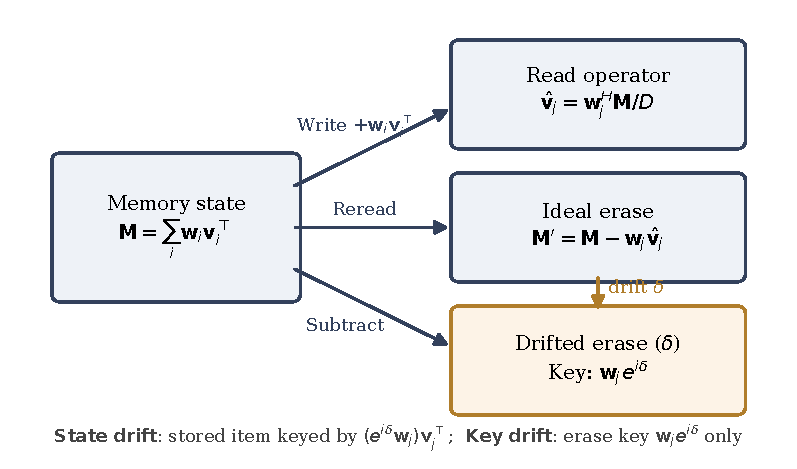
\includegraphics[width=0.78\textwidth]{fig1_memory_diagram.pdf}
  \caption{Write, read, and erase operators of the matrix-valued associative memory, illustrating the two controlled drift locations: phase drift of the erase key at unbinding time (key drift) and write-time phase offset on the target association followed by reference-clock mismatch during unbinding (state drift).}
  \label{fig:diagram}
\end{figure}

\subsection{Controlled drift locations}

Two controlled phase interventions are evaluated (Figure~\ref{fig:diagram}):
\begin{enumerate}
  \item \textbf{Key drift} ($\w_j \to \tilde{\w}_j = \w_j e^{i\delta}$): The associations are stored without perturbation. During erasure, local-oscillator drift changes the erase key to $\tilde{\w}_j$. Both the reread estimate $\vhat_j = \tilde{\w}_j^H \M / D$ and the subtractive unbinding use the drifted key:
  \begin{equation}
  \M' = \M - \tilde{\w}_j \vhat_j.
  \end{equation}
  \item \textbf{State drift}: We use \emph{state drift} to denote a write-time phase offset attached to the target association, followed by a mismatch between the stored phase coordinate used for rereading and the reference coordinate used for unbinding. Specifically, the target item is stored as $(e^{i\delta} \w_j) \vb_j^\top$. The erase operation rereads using the item's stored coordinate $\tilde{\w}_j = e^{i\delta}\w_j$ to obtain a value estimate, $\vhat_j = \tilde{\w}_j^H \M / D$, but performs unbinding with the unperturbed reference-clock key $\w_j$:
  \begin{equation}
  \M' = \M - \w_j \vhat_j.
  \end{equation}
\end{enumerate}

Query readout is always evaluated with the unperturbed reference key $\w_j$. For the complex channel, the post-erase query residual is $\mathbf{r}_j = \w_j^H \M' / D$. For the real channel, real truncation is applied both during reread ($\vhat_j \leftarrow \operatorname{Re}(\vhat_j)$) and at query readout: $\mathbf{r}_j = \operatorname{Re}(\w_j^H \M' / D)$. Truncation is applied at both locations because the trained readout head consumes real-truncated representations end-to-end; single-sided variants define different operators and are not evaluated here.

\section{Closed-form residual laws}\label{sec:laws}

Under the independent random-key model (i.i.d.\ unit-modulus entries with uniform phases), the effect of the number of interfering associations is captured by $c=(n-1)/D$, following classical distributed capacity scaling \citep{plate1995holographic,kanerva2009hyperdimensional,frady2018theory}. For the pooled residual energy normalized by the pooled target energy $L = \sum_i \|\mathbf{r}_i\|^2 / \sum_i \|\vb_i\|^2$, the expected values under random unit-modulus keys are described by four closed-form, fit-free expressions:
\begin{align}
L_{\text{key, complex}}(\delta) &= 0, \label{eq:law_kc} \\
L_{\text{state, complex}}(\delta) &= 2(1-\cos\delta)\,(1+c), \label{eq:law_sc} \\
L_{\text{key, Re}}(\delta) &= \sin^4\delta + \frac{c}{4}\bigl(1-\cos 2\delta\bigr), \label{eq:law_kr} \\
L_{\text{state, Re}}(\delta) &= (1-\cos\delta)^2 + c\,(1-\cos\delta). \label{eq:law_sr}
\end{align}

\begin{figure}[t]
  \centering
  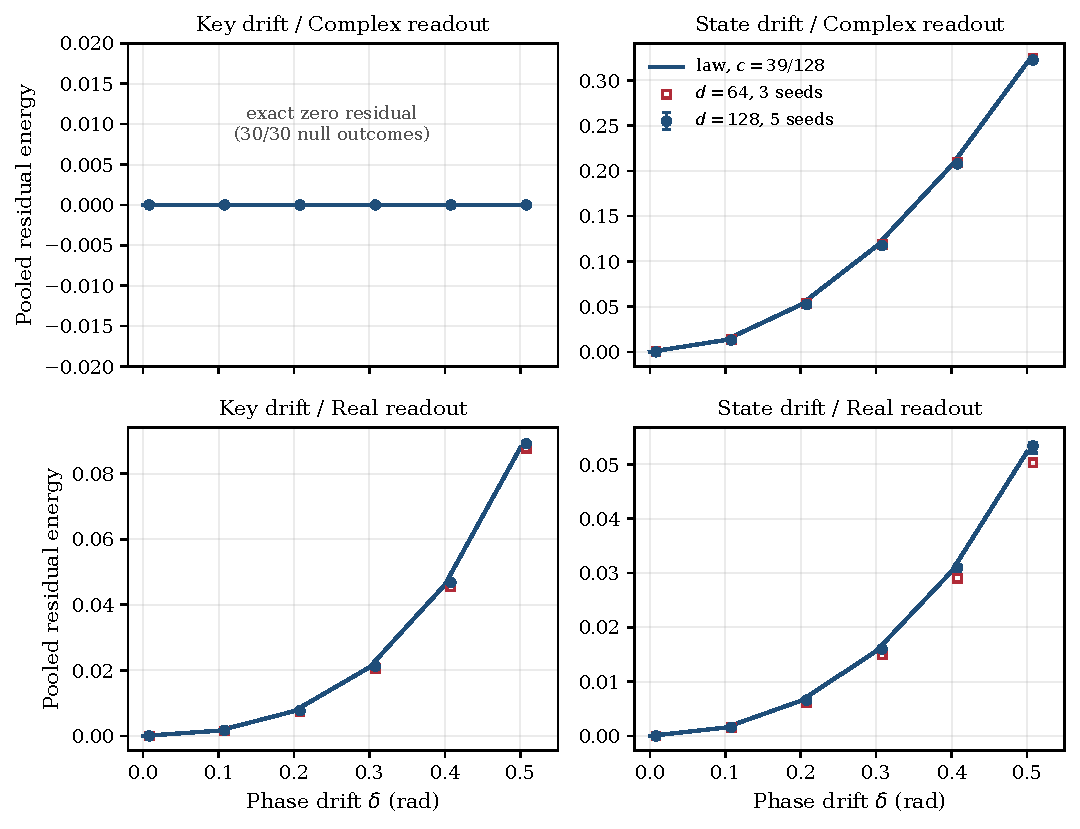
\includegraphics[width=0.92\textwidth]{fig2_residual_laws.pdf}
  \caption{Measured pooled residual energy versus the four closed-form laws across drift values $\delta \in \{0.0, 0.1, 0.2, 0.3, 0.4, 0.5\}$. Closed circles: $D=128$, five seeds (median with min--max bars). Open squares: $D=64$, three seeds. The key/complex cell produces an algebraically zero residual under the idealized operator (and numerically null residuals below $\varepsilon_{\text{null}}=10^{-4}$ across all 30 tested runs: five seeds $\times$ six drift magnitudes at $D=128$).}
  \label{fig:laws}
\end{figure}

\paragraph{Derivation sketch for Eq.~\eqref{eq:law_sc}.} Under state drift, the reread estimate with stored coordinate $\tilde{\w}_j = e^{i\delta}\w_j$ gives $\vhat_j = \vb_j^\top + \frac{e^{-i\delta}}{D}\sum_{k \ne j}\w_j^H \w_k \vb_k^\top$: the target phase cancels because the estimate is read with the item's own stored coordinate. Subtracting $\w_j \vhat_j$ produces post-erase state $\M' = (e^{i\delta}-1)\w_j \vb_j^\top + \sum_{k \ne j} \w_k \vb_k^\top - \w_j \frac{e^{-i\delta}}{D}\sum_{k \ne j} \w_j^H \w_k \vb_k^\top$. Reading $\M'$ with reference key $\w_j$ returns target residual $(e^{i\delta}-1)\vb_j^\top$ and crosstalk $(1-e^{-i\delta})\frac{1}{D}\sum_{k \ne j}(\w_j^H \w_k)\vb_k^\top$. Squared residual norms are summed over stored items before taking expectations (matching the definition of the pooled estimator). Substituting $\mathbb{E}[|\w_j^H \w_k|^2] = D$ for $k \ne j$ and $\sum_j \sum_{k \ne j} \|\vb_k\|^2 = (n-1)\sum_k \|\vb_k\|^2$ yields
\begin{equation}
\frac{\sum_j \mathbb{E}[\|\mathbf{r}_j\|^2]}{\sum_j \|\vb_j\|^2} = |e^{i\delta}-1|^2 + |1-e^{-i\delta}|^2 \frac{n-1}{D} = 2(1-\cos\delta)(1+c),
\end{equation}
with no equal-norm assumption on the target vectors.

\paragraph{Key/complex null residual.} Under coherent key drift, $\M' = \M - \tilde{\w}_j (\tilde{\w}_j^H \M / D)$ is algebraically an exact orthogonal projection onto the subspace orthogonal to $\tilde{\w}_j$, eliminating the target component identically ($L=0$ in the algebraic model). In numerical experiments, all 30 runs at $D=128$ ($5$ seeds $\times$ $6$ drift magnitudes) produced residuals below the pre-specified null-guard threshold $\varepsilon_{\text{null}} = 10^{-4}$. In contrast, the remaining three cells retain structured residuals whose energy alone does not reveal whether a decoder can recover the forgotten value.

\section{Write stability}\label{sec:stability}

The normalized-delta comparison arm requires bounded write dynamics. The corrective delta rule updates the model's state matrix $\St$ (distinct from the analytic memory $\M$ above) according to
\begin{equation}
\St_t = \St_{t-1} + \beta\, \mathbf{k}_t \bigl(\mathbf{v}_t^\top - \mathbf{k}_t^\top \St_{t-1}\bigr),
\end{equation}
where $\mathbf{k}_t$ and $\mathbf{v}_t$ are column vectors; for complex keys and states, transposes are replaced by conjugate transposes.
Under a first-order directional approximation assuming quasi-orthogonal keys, the error dynamics along direction $\mathbf{k}_t$ follow the scalar recursion
\begin{equation}
s_t = \bigl(1 - \beta\|\mathbf{k}_t\|^2\bigr) s_{t-1} + \beta\, q_t,
\end{equation}
where $q_t$ represents crosstalk interference. The homogeneous dynamics are stable if and only if $|1 - \beta\|\mathbf{k}_t\|^2| < 1$, which requires $0 < \beta\|\mathbf{k}_t\|^2 < 2$.

With $\beta=1$ and unnormalized key embeddings initialized such that $\|\mathbf{k}_t\|^2 \approx 8$, the directional feedback multiplier is approximately $1 - 8 = -7$. The task uses a finite key vocabulary that recurs across updates, so this per-direction multiplier is applied repeatedly along shared directions. Under the quasi-orthogonality approximation these directions evolve independently, and their error components compound: $\|\St\|$ grows to $10^{11}$--$10^{12}$ within the first epochs, and the unnormalized corrective baseline fails. Normalizing the keys ($\|\mathbf{k}_t\|_2^2=1$) yields a normalized-key delta update \citep{widrow1960adaptive,widrow1985adaptive}; for $0 < \beta < 2$, this ensures $|1-\beta|<1$ and keeps the directional homogeneous dynamics inside the unit disk, maintaining bounded state norm and achieving stable retrieval (Figure~\ref{fig:stability}).

This stability derivation provides an explanatory mechanism for why unnormalized closed-loop delta writes diverge without key normalization. It does not imply that all contemporary delta-rule architectures are unstable, as modern implementations typically incorporate RMSNorm, LayerNorm, or decay gating \citep{yang2024deltanet,yang2025gateddelta}. In contrast, the open-loop superposition write possesses no corrective feedback loop and does not exhibit the corrective-feedback instability analyzed here.

\begin{figure}[t]
  \centering
  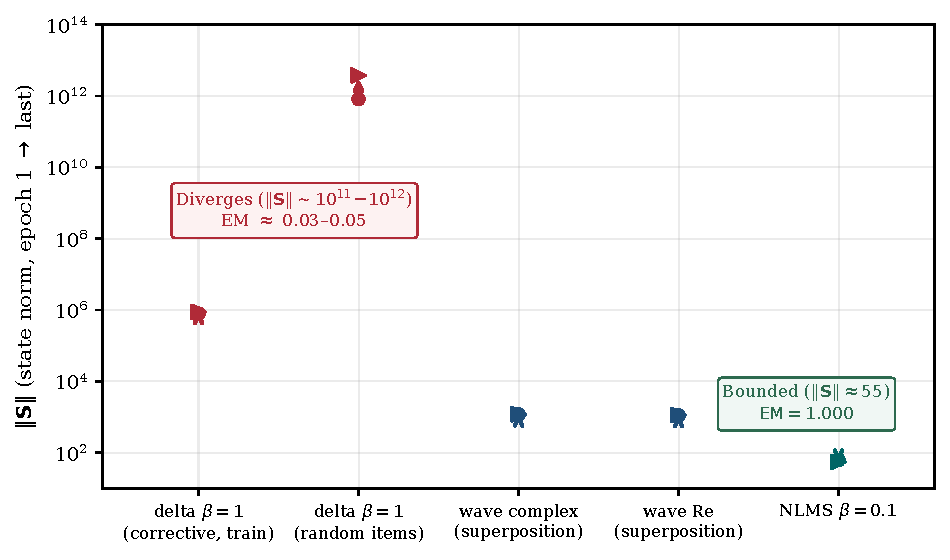
\includegraphics[width=0.78\textwidth]{fig5_write_stability.pdf}
  \caption{State-norm evolution (log scale, epoch 1 to final epoch). Corrective delta with $\beta=1$ diverges ($\mathrm{EM}\approx 0.03$--$0.05$). Superposition writes (wave complex, wave Re) remain bounded. Normalized-key delta with $\beta=0.1$ maintains a bounded state norm and reaches $\mathrm{EM}=1.000$.}
  \label{fig:stability}
\end{figure}

\section{Experiments}\label{sec:experiments}

The evaluation progressed from synthetic algebra checks to fully trained recurrent models. The scale-matched experiment evaluated $D=64$ ($n=20$ pairs, associative load $c=19/64 \approx 0.2969$, three seeds) and $D=128$ ($n=40$ pairs, associative load $c=39/128 \approx 0.3047$, five seeds) across a drift grid $\delta \in \{0.0, 0.1, 0.2, 0.3, 0.4, 0.5\}$. A discrete vocabulary of 105 tokens was used (48 key tokens, 48 value tokens, and delimiter markers); the token vocabulary is used strictly to construct controlled associative sequences and is not intended as a natural-language modeling benchmark. Each arm and seed evaluated 320 forgetting events. For inferential comparisons, the random seed---not the individual forgetting event---was treated as the independent experimental unit. The unit-modulus key codebook is shared across all seeds (using a fixed generation seed). Seed-level variability therefore reflects parameter initialization and dataset sampling (training/validation pairs and probe events), not resampling from the random-key ensemble underlying the closed-form expectations. Within each run, the probe aggregates 320 events spanning many query--key realizations.

The primary residual metric was pooled across events:
\begin{equation}
L = \frac{\sum_i \|\mathbf{r}_i\|^2}{\sum_i \|\mathbf{v}_i\|^2},
\end{equation}
which avoids the heavy-tail variance of averaging per-example ratios when target vector norms vary. A linear ridge-regression probe ($\alpha=0.1$) used a within-model 75\%/25\% train--test split ($n=240$/$n=80$) to measure whether the post-erase query residual vector $\mathbf{r}_j$ retained sufficient structure to decode the continuous target vector $\vb_j \in \R^D$. At test time, continuous predictions $\hat{\mathbf{v}}$ were mapped to the value vocabulary by nearest cosine similarity to codebook vectors, and exact match was recorded when the recovered token matched the true target. Retrieval selectivity was evaluated across retained and erased pairs:
\begin{equation}
\text{Selectivity} = \mathrm{EM}_{\text{alive}} - \mathrm{EM}_{\text{erased}}.
\end{equation}
Erased-item exact match (EM) was computed only for nonzero residuals; residuals below the guard threshold $\varepsilon_{\text{null}} = 10^{-4}$ were instead classified as numerically null. The threshold is set well above the floating-point noise floor of the computation.

At $D=128$, all 15 seed--arm combinations reached $\mathrm{EM}=1.000$; at $D=64$, the nine seed--arm combinations trained to saturation ($\mathrm{EM} \ge 0.99$ in every recorded run). Because the synthetic associative task saturates at this scale, EM serves as a validation sanity check rather than the primary evidence.

\section{Results}\label{sec:results}

Table~\ref{tab:deviations} reports maximum absolute deviations between measured pooled residuals and the closed-form predictions across cells and dimensions, recomputed directly from the frozen JSON artifacts by \texttt{verify\_numbers.py}. At $D=64$, the maximum absolute deviation is $0.0094$; at $D=128$, it is $0.0049$. Both values remain below the pre-specified consistency tolerance of $0.02$ (Figure~\ref{fig:laws}); ensemble-calibrated standard deviations (Supp.~G) place these maxima at approximately one standard deviation of the random-key ensemble.

\begin{table}[t]
  \centering
  \caption{Maximum absolute deviation $|\text{measured} - \text{predicted}|$ over seeds and the drift grid per cell, under the pooled estimator (recomputed from frozen artifacts). Key/complex residuals are recorded as numerically null below $\varepsilon_{\text{null}}=10^{-4}$.}
  \label{tab:deviations}
  \vspace{0.5em}
  \begin{tabular}{@{}llcc@{}}
    \toprule
    perturbation & readout channel & $D=64$ & $D=128$ \\
    \midrule
    key drift   & complex (algebraic zero) & $<10^{-4}$ & $<10^{-4}$ \\
    state drift & complex: $2(1{-}\cos\delta)(1{+}c)$ & 0.0094 & 0.0049 \\
    key drift   & real (Re): $\sin^4\delta + c(1{-}\cos 2\delta)/4$ & 0.0016 & 0.0018 \\
    state drift & real (Re): $(1{-}\cos\delta)^2 + c(1{-}\cos\delta)$ & 0.0015 & 0.0018 \\
    \midrule
    \multicolumn{2}{@{}l}{Pre-specified consistency tolerance} & $\le 0.02$ & $\le 0.02$ \\
    \bottomrule
  \end{tabular}
\end{table}

At approximately matched load ($c \approx 0.30$, differing by $\approx 2.6\%$ between dimensions), the three non-trivial cells demonstrate close agreement across dimensions, with a maximum cross-scale difference of $0.0064$ under the stored pairing convention (below $0.011$ under every aggregation convention examined; Figure~\ref{fig:load}). Of this observed maximum, $0.0019$ at $\delta=0.5$ is attributable to the residual load mismatch alone under the state/complex law; the remainder reflects finite-sample and optimization variability. Inverting these laws on the measured pooled residuals recovers the generating load $c=(n-1)/D$ at both scales ($c=39/128 \approx 0.3047$ at $D=128$ and $c=19/64 \approx 0.2969$ at $D=64$); because the laws are linear in $c$, this inversion is a consistency check rather than independent validation. The key/complex cell is identically zero for every load and therefore carries no information about load dependence; its residuals remain numerically null below $\varepsilon_{\text{null}}$ at both scales.

The key/complex cell produced algebraically zero and numerically null residuals below $\varepsilon_{\text{null}}$ in all 30 tested runs. The other cells showed nonzero residuals that supported linear decoding under the specified within-model protocol, despite their low energy leakage. Specifically, at $D=128$, the key/Re residual reaches only $\approx 0.0016$ pooled energy at $\delta=0.1$, yet the ridge decoder recovers the erased value in about $5\%$ of test events on average across seeds (range $1.3\%$--$7.5\%$); chance level for nearest-token decoding over the 48-value vocabulary is $1/48 \approx 2.1\%$, so low-$\delta$ decoding stays within a few times chance, and the dissociation claim rests on the mid-to-high drift range. Decodability remains low until $\delta\approx0.25$ and increases substantially by $\delta\approx0.4$, whereas energy increases smoothly across the entire range (Figure~\ref{fig:decodability}). This disparity demonstrates why forgetting evaluation requires both operator-level residual metrics and functional decoding probes.

\begin{figure}[t]
  \centering
  \begin{minipage}[t]{0.48\textwidth}
    \centering
    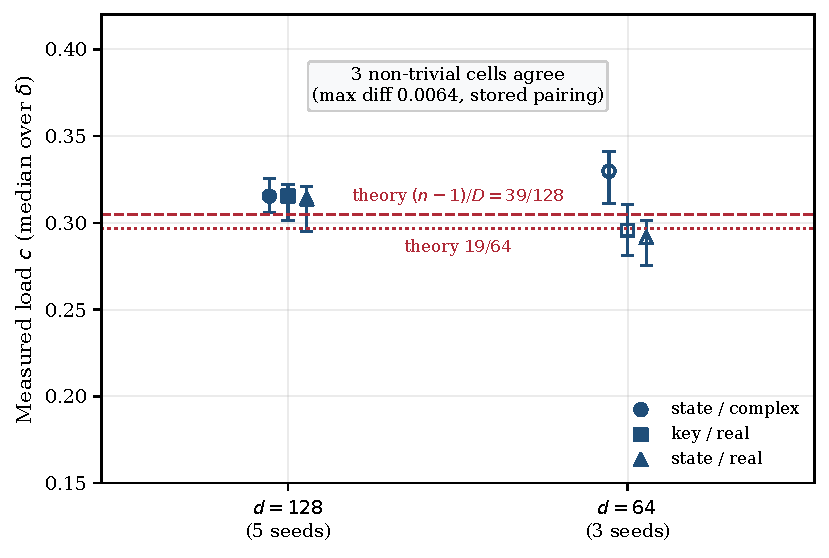
\includegraphics[width=\textwidth]{fig3_load_scaling.pdf}
    \caption{Measured load $c$ (median over drift values $\delta > 0$, with min--max bars) inverted from the three non-zero laws versus expected load $(n-1)/D$. Cross-dimensional agreement: maximum cell difference $0.0064$ for the three non-trivial cells.}
    \label{fig:load}
  \end{minipage}\hfill
  \begin{minipage}[t]{0.48\textwidth}
    \centering
    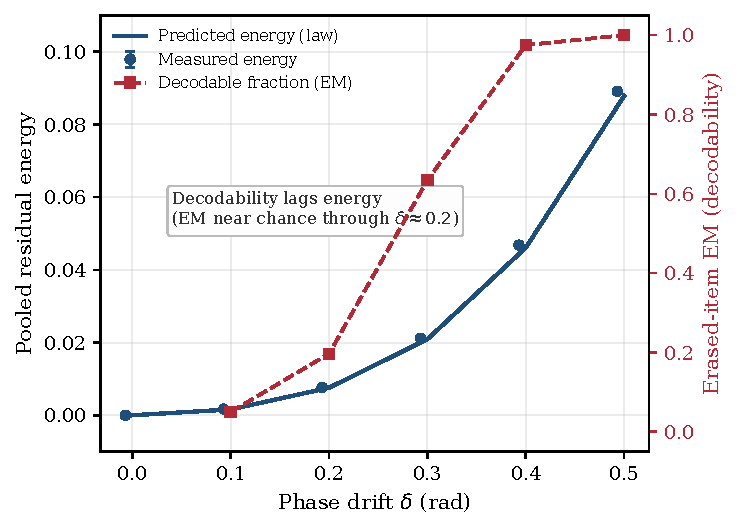
\includegraphics[width=\textwidth]{fig4_energy_vs_decodability.pdf}
    \caption{Key/Re cell at $D=128$: pooled residual energy versus erased-item EM (ridge decodability). Erased-item EM is undefined at $\delta=0$ (residuals are null-guarded) and stays within a few times chance through $\delta\approx0.2$, rising clearly by $\delta=0.4$; pooled energy grows smoothly throughout.}
    \label{fig:decodability}
  \end{minipage}
\end{figure}

The unnormalized $\beta=1$ corrective delta baseline failed to train because its write updates diverged (Section~\ref{sec:stability}). Normalized delta writes trained stably and produced a small mean difference in retrieval selectivity (wave complex minus normalized delta: $-0.0031$; the normalized-delta arm retains slightly more selectivity), with a two-sided $90\%$ confidence interval (TOST at $\alpha=0.05$; per-seed selectivity differences paired across arms, Student-$t$ interval with four degrees of freedom) of $[-0.0206,\,0.0144]$ (Figure~\ref{fig:tost}). The two arms are compared under their respective deployed training recipes, which differ in budget (Section~\ref{sec:experiments}; Supp.~F), so the comparison concerns operator-plus-recipe composites; isolating the write operators alone would require budget-matched retraining. Because the lower confidence bound crosses the equivalence margin $-\varepsilon=-0.02$ by $0.0006$ under $n=5$ seeds, the result is reported as inconclusive with respect to formal equivalence within margin $\varepsilon=0.02$.

\begin{figure}[t]
  \centering
  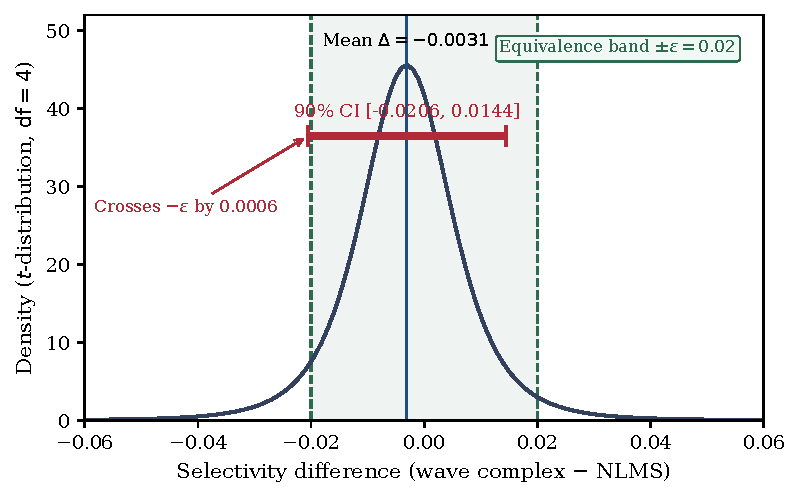
\includegraphics[width=0.62\textwidth]{fig6_tost.pdf}
  \caption{Two one-sided $t$-test (TOST at $\alpha=0.05$, $90\%$ CI) on retrieval selectivity between wave complex and normalized delta ($\varepsilon=0.02$, $n=5$ seeds). Mean difference: $-0.0031$; $90\%$ CI: $[-0.0206,\,0.0144]$. The confidence interval crosses $-\varepsilon$ by $0.0006$.}
  \label{fig:tost}
\end{figure}

\section{Relation to prior work}\label{sec:related}

The memory construction sits within a long associative-memory lineage: correlation-matrix memories \citep{kohonen1972correlation,willshaw1969nonholographic}, the Hopfield network and its signal-to-noise analyses of crosstalk \citep{hopfield1982neural}, dense associative extensions \citep{krotov2016dense}, and the modern Hopfield--attention bridge \citep{ramsauer2021hopfield}. Within this tradition, the residual laws of Section~\ref{sec:laws} are second-moment statements about crosstalk, akin to classical SNR computations; what is added here is an operator- and channel-resolved characterization of what erasure leaves behind. The superposition--matched-filter--unbinding formalism belongs to the holographic reduced-representation and vector-symbolic architecture traditions \citep{plate1995holographic,kanerva2009hyperdimensional,gayler2003vector}, with capacity characterized by \citet{frady2018theory} and factorization analyzed by \citet{frady2020resonator}; complex-valued phasor memories trace back to \citet{noest1988phasor} and reappear in recent phase-associative sequence models \citep{vishwakarma2026phaseassociative}, which share the complex outer-product state but target language modeling at scale rather than erase-residual characterization.

In the fast-weight literature, the mechanism dates to \citet{schmidhuber1992learning} and returned as attention by \citet{ba2016using}; linear attention was established by \citet{katharopoulos2020transformers}, with the delta rule cast as a fast-weight programmer by \citet{schlag2021fastweight}. Delta-rule linear attention and its parallel forms \citep{yang2024deltanet}, multiplicative decay architectures---RWKV \citep{peng2023rwkv}, RetNet \citep{sun2023retentive}, Mamba and structured state-space duality \citep{gu2023mamba,dao2024transformers}, gated linear attention \citep{yang2024gla}---constitute the modern landscape in which forgetting is implemented primarily through multiplicative decay gating rather than subtractive erasure. Two test-time-memory lines are adjacent but mechanistically distinct: TTT layers update their memory state by gradient steps at inference time \citep{sun2024ttt}, and Titans adds a surprise-gated neural long-term memory alongside attention \citep{behrouz2025titans}. Two fine-grained delta-rule lines are closest to this work: Kimi Delta Attention extends Gated DeltaNet \citep{yang2025gateddelta} with finer-grained decay gating \citep{kimi2025linear}, and Comba analyzes bilinear delta-rule recurrences through closed-loop control theory \citep{hu2025comba}, a control-theoretic reading complementary to the LMS analysis of Section~\ref{sec:stability}. Gated DeltaNet-2 \citep{hatamizadeh2026gateddeltanet2} further decouples erasing from writing through channel-wise erase and write gates; the present laws characterize subtractive projection-style erasure, and deriving their analogues under multiplicative, channel-wise erasure is an open direction. As a distant analogue in deployed systems, rotary position embeddings attach position-dependent phases to keys whose write-time and read-time values differ \citep{su2021roformer}; unlike the controlled drift studied here, those rotations are deterministic and compensated at readout. Recall-centric evaluations in linear-attention systems \citep{arora2024simplelinear,arora2024zoology} complement the operator-level protocol studied here. Classical LMS/NLMS adaptive filtering theory \citep{widrow1960adaptive,widrow1985adaptive} provides the foundation for the directional stability analysis in Section~\ref{sec:stability}.

The framework is also related to machine unlearning and privacy research \citep{guo2020certified,bourtoule2021machine,sekhari2021remember}, but addresses a different problem: machine-unlearning methods typically evaluate parameter-space indistinguishability from a retrained model, whereas the present study measures residual state structure and separates energetic leakage from functional recoverability in recurrent memory states.

The scope of novelty is specifically delimited: establishing a forgetting-centric evaluation protocol, formalizing the divergence between energetic and functional leakage, deriving the four-way drift/channel residual laws, and empirically validating these closed-form laws in trained recurrent memories under approximately matched associative load.

\section{Limitations}\label{sec:limits}

The present study uses synthetic key--value associative tasks, fixed codebooks, real-valued targets, an explicit matrix state requiring $O(D^2)$ parameters per layer, and controlled drift interventions. The closed-form laws assume independent unit-modulus random keys and single-item phase perturbations; learned codebooks, correlated multi-item drift, natural-language sequence modeling, and hardware throughput benchmarking represent avenues for future research. Statistical comparisons between arms are limited by the available seed count ($n=5$ at $D=128$, $n=3$ at $D=64$); no prospective power analysis was conducted, although a post-hoc calculation from the observed dispersion (per-seed standard deviation $\approx 0.018$) indicates that $n \approx 8$ paired seeds would provide approximately $90\%$ power to establish equivalence at the margin $\varepsilon = 0.02$. The cross-scale comparison holds the associative load approximately matched (within $\approx 2.6\%$; exact matching would require $n=39$ pairs at $D=128$), and a systematic sweep of $c$ at fixed $D$ has not been performed. Erasure through multiplicative, channel-wise decay or erase gates---as deployed in recent gated delta architectures \citep{yang2025gateddelta,hatamizadeh2026gateddeltanet2}---is not modeled here; the present laws characterize subtractive projection-style erasure.

\section{Conclusion}\label{sec:conclusion}

Selective forgetting in recurrent associative memory cannot be characterized adequately by retrieval accuracy alone: a residual can carry almost no energy yet remain partially decodable. Within fixed-codebook matrix-valued memories, what erasure leaves behind is governed by four closed-form laws with no free parameters, verified on trained models at two scales under approximately matched load; exact erasure reflects alignment between the erase key and the readout key rather than the operator family itself. Two boundaries define the present scope: erasure here is subtractive projection, whereas deployed gated architectures forget primarily through multiplicative decay; and the equivalence between superposition and normalized-delta operators remains statistically inconclusive with only five seeds. Addressing both limitations---deriving multiplicative-erasure residual laws and conducting an adequately powered equivalence test---is the natural next step for this line of research.

\section*{Reproducibility}

Code, configurations, checkpoints, raw JSON outputs, execution logs, and verification scripts are released in the open repository \url{https://github.com/01javierescobar/operator-specific-forgetting}, archived with DOI \href{https://doi.org/10.5281/zenodo.22051928}{10.5281/zenodo.22051928}. The frozen reference commit is \texttt{cec4ffe}, tagged \texttt{lab-radioactivo-v1}. All quantitative values in this manuscript are recomputed directly from the frozen JSON artifacts by \texttt{paper/verify\_numbers.py}; all figures are regenerated by \texttt{paper/make\_figures.py}. The primary trained-model gate (O05) was executed on two NVIDIA T4 GPUs (Kaggle kernel \texttt{javierezcobar/onda-o05}, 5.44~h, 15 runs).

\section*{Use of AI tools}

AI-assisted tools (large language models) were used throughout the research process for code development, experimental design iteration, debugging, and adversarial verification of intermediate claims across the O01--O05 protocol. All mathematical derivations, experimental protocols, quantitative results, and scientific conclusions were validated by the author. The AI tools are not listed as authors and bear no responsibility for the content of this manuscript.

\bibliographystyle{plainnat}
\bibliography{references}

\end{document}